\documentclass[12pt]{article}

\usepackage[polish]{babel}
\usepackage{csquotes}
\usepackage[a4paper,top=2.5cm,bottom=2.5cm,left=3cm,right=2cm]{geometry}
\usepackage{indentfirst}
% Useful packages
\usepackage{lipsum}
\usepackage{amsmath}
\usepackage{graphicx}
\usepackage[colorlinks=true, allcolors=blue]{hyperref}
\usepackage{float}
\usepackage{fontspec}
\setmainfont{Times New Roman}
\setlength{\parindent}{1.25cm}
\linespread{1.5}
\setlength{\parskip}{6pt}
\usepackage[sorting=none]{biblatex}
\addbibresource{bibliography.bib}
\hypersetup{linkcolor=black}
\usepackage[all]{hypcap}
\addto\captionspolish{\renewcommand{\figurename}{Rys.}}
\addto\captionspolish{\renewcommand{\tablename}{Tab.}}
\renewcommand{\tableautorefname}{Tab.} % PS
\renewcommand{\figureautorefname}{Rys.} % PS
\renewcommand{\listfigurename}{Spis rysunków}
\renewcommand{\listtablename}{Spis tabel}

\newcommand{\image}[3][16cm]{
\begin{figure}[H]
    \centering
    \includegraphics[width=#1]{imgs/#2}
    \caption{#3}
    \label{img:#2}
\end{figure}
}

\begin{document}

\newpage
\clearpage
\tableofcontents

\newpage
\addcontentsline{toc}{section}{Wstęp}
\section*{Wstęp}

Zarządzanie i obsługa wydarzeń od zawsze były wymagającym przedsięwzięciem, stanowiącym wyzwanie dla jednostek oraz instytucji, które pragną dostarczyć efektywne i satysfakcjonujące doświadczenia uczestnikom. Rola wydarzeń w społeczeństwie ewoluowała z prostych zgromadzeń do złożonych i wielowarstwowych struktur, wymagających precyzyjnej koordynacji, ścisłego planowania i efektywnego zarządzania zasobami. W rezultacie organizacja wydarzeń stała się procesem złożonym, który wymaga zaangażowania wielu osób i instytucji, a także wykorzystania specjalistycznych narzędzi i rozwiązań.

Wraz z dynamicznym postępem technologicznym, rozwija się również dziedzina narzędzi wspomagających proces organizacyjny. Nowoczesne aplikacje mobilne oraz platformy internetowe i rozwiązania informatyczne stają się integralną częścią skutecznego zarządzania wydarzeniami. Niemniej jednak obecna oferta na rynku skupia się głównie na potrzebach dużych przedsiębiorstw, które regularnie organizują wydarzenia o znacznej skali, takie jak międzynarodowe koncerty czy masowe festiwale.

Wspomniane rozwiązania, choć wysoce efektywne w specyficznych kontekstach, cechują się również kosztami użytkowania oraz skomplikowaną strukturą, co stawia dodatkowe wyzwania przed mniejszymi organizacjami. W szczególności uczelnie czy organizacje studenckie, które często są inicjatorami wydarzeń o mniejszym zakresie, takich jak jednodniowe konferencje czy warsztaty, napotykają trudności w dostosowaniu ogólnodostępnych narzędzi do swoich specyficznych potrzeb.

Deficyt dostępu do dedykowanych rozwiązań stanowi dla mnie inspirację do stworzenia nowej aplikacji, dostosowanej do specyficznych potrzeb mniejszych organizacji. Mój cel to usprawnienie procesu organizacyjnego oraz podniesienie dostępności i efektywności dla tego typu podmiotów. W tym celu postanowiłem stworzyć nową aplikację, która pozwoli na zarządzanie i obsługę  wydarzeń w sposób prosty i intuicyjny, a także dostosowany do specyficznych potrzeb mniejszych organizacji.
\newpage

\addcontentsline{toc}{section}{Cel i zakres pracy}
\section*{Cel i zakres pracy}
Celem niniejszej pracy dyplomowej jest zaprojektowanie oraz implementacja aplikacji na wiele platform, która w znaczny sposób usprawni procesy związane z zarządzaniem i obsługą wydarzeń.

Zakres pracy obejmuję stworzenie w pełni działającej aplikacji internetowej, która będzie miała możliwość rejestracji i logowania użytkowników za pomocą konta Google, zapisu na wybrane wydarzenia objęte limitem uczestników warsztatów. Aplikacja będzie posiadała również panel administracyjny, który będzie umożliwiał zarządzanie użytkownikami i wydarzeniami, dodawanie nagród rzeczowych, generowanie kodów QR dla każdego z wydarzeń, które będą służyły do potwierdzenia obecności uczestnika na wydarzeniu bądź będą wynagradzać uczestnika punktami za zeskanowanie kodu. W aplikacji mobilnej użytkownik będzie mógł zeskanować kod QR, będzie mógł sprawdzić posiadaną ilość punktów oraz podstawowe informacje o warsztatach i nagrodach. Dodatkowo organizator przy pomocy aplikacji mobilnej będzie mógł wyłonić zwycięzców nagród z systemu losującego na podstawie punktów zdobytych przez uczestników. Organizator oraz wolontariusz będą posiadać możliwość potwierdzania obecności danego użytkownika na wydarzeniu przy pomocy skanera, który będzie zaimplementowany w aplikacji mobilnej.



\newpage

\section{Rozdział z dziedziny pracy - część teoretyczna}
\subsection{Rys historyczny}
Wydarzenia od zawsze stanowiły integralną część życia społecznego. Początkowo jedyną formą informowania o odbywających się wydarzeniach była forma  ustna. Wraz z rozwojem cywilizacji ludzkość zaczęła posługiwać się pismem, co umożliwiło zapisywanie informacji o wydarzeniach i sporządzanie listy uczestników. Umożliwiło to także precyzyjne planowanie oraz dokładne dokumentowanie uroczystości przez osoby wykształcone, posługujące się pismem.

Kluczowym momentem w rozwoju wydarzeń było wynalezienie druku w 1450 roku przez Jana Gutenberga. Pozwoliło to na zwiększenie ilości materiałów informacyjnych oraz ich dystrybucję i archiwizację. Wraz z rozwojem technologii druku, w 1609 roku w Strasburgu powstała pierwsza gazeta, co przyczyniło się do tworzenia powierzchni reklamowych dla wszelkich wydarzeń oraz zwiększyło dostęp do informacji i zainteresowanie społeczeństwa. \autocite{gazeta}

Rewolucja przemysłowa na przełomie XVIII i XIX wieku przyczyniła się do znaczących zmian w zakresie zarządzania i organizacji wydarzeń. Dostęp informacji dla społeczeństwa został znacząco zwiększony, co przyczyniło się do rozwoju mediów oraz reklamy. Masowo drukowane ulotki i gazety znacznie zwiększyły zasięg informacji o wydarzeniach, co przyczyniło się do zwiększenia liczby uczestników. Obecność afiszu teatralnego z 1799 roku (\autoref{rys:afisz}) stanowi doskonały przykład, ilustrujący, jak technologiczne innowacje wpłynęły na zwiększenie zasięgu informacji o wydarzeniach i sprzyjały wzrostowi liczby uczestników, tworząc dynamiczne środowisko kulturalne i społeczne.

\begin{figure} [H]
    \begin{center}
    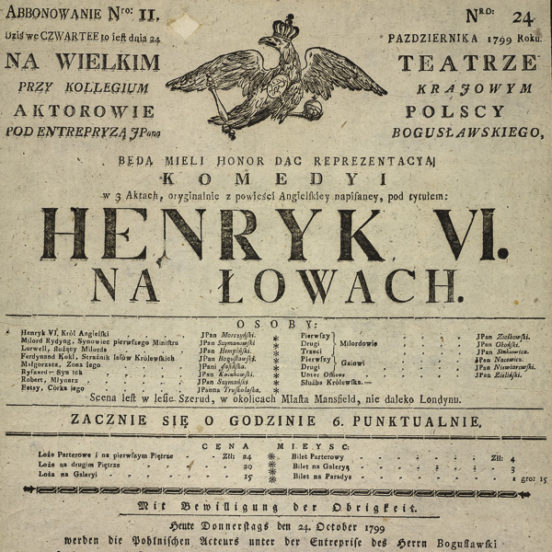
\includegraphics[scale=0.20]{imgs/afisz.jpg}
    \end{center}
    \caption{Afisz teatralny z 1799 roku \autocite{polona}}
    \label{rys:afisz}
    \end{figure}

W końcówce XX wieku wraz z pojawieniem się ogólnodostępnych technologii komputerowych pojawiły się pierwsze systemy informatyczne wspomagające organizację wydarzeń. Wraz z rozwojem Internetu i technologii mobilnych, systemy informatyczne stały się coraz bardziej dostępne i popularne, co umożliwiło ich wykorzystanie w organizacji wydarzeń np. poprzez użycie kodów QR do sprawdzania obecności na wydarzeniu. Obecnie systemy informatyczne stanowią integralną część organizacji wydarzeń, a ich rozwój jest dynamiczny i nieustanny.
\subsection{Przegląd istniejących rozwiązań}
Obecnie na rynku oferowanych jest już kilka rozwiązań, które pozwalają  w mniejszym lub większym stopniu na zarządzanie i obsługę wydarzeń.

Przedstawione poniżej rozwiązania częściowo wykonują te same zadania. Różnią się od siebie jednak zastosowanymi technologiami, sposobem działania oraz dostępnymi funkcjonalnościami czy podejściem do problemu. Ważnym aspektem jest również cena, która w przypadku niektórych rozwiązań jest bardzo wysoka.

\subsubsection{Meetup}
\input{sections/chapters/theory/solutions/meetup.tex}
\subsubsection{Eventbrite}
\input{sections/chapters/theory/solutions/eventbrite.tex}
\subsubsection{Event Espresso}
\input{sections/chapters/theory/solutions/eventespresso.tex}
\subsubsection{Bizzabo}
\input{sections/chapters/theory/solutions/bizzabo.tex}
\newpage

\section{Zakres użytych technologii i opis wykorzystywanych narzędzi}
W niniejszej pracy zastosowano technologie, które spełniają ściśle określone kryteria, zgodnie z zainteresowaniami autora. Wybrane technologie zostały ocenione pod kątem poniższych parametrów:

\begin{itemize}
    \item \textbf{Otwarty kod źródłowy:} Wybrane technologie opierają się na otwartym kodzie źródłowym, co umożliwia pełen dostęp, analizę, oraz ewentualne dostosowanie do indywidualnych potrzeb.
    
    \item \textbf{Darmowe:} Wszystkie technologie są dostępne bez dodatkowych opłat, co jest istotne z perspektywy ekonomicznej.
    
    \item \textbf{Popularne:} Wybór technologii uwzględniał ich popularność w branży, co zapewnia szeroką dostępność dokumentacji oraz wsparcie społeczności.
    
    \item \textbf{Duża społeczność:} Wykorzystane technologie cieszą się uznaniem w społeczności, co gwarantuje aktywną wymianę wiedzy oraz dostępność rozwiązań problemów.
    
    \item \textbf{Ogólnodostępne:} Technologie są powszechnie dostępne dla użytkowników o różnym poziomie doświadczenia, co ułatwia ich adaptację.
    
    \item \textbf{Regularne aktualizacje:} Wybrane technologie są systematycznie aktualizowane, co zapewnia korzystanie z najnowszych funkcji oraz zabezpieczeń.
\end{itemize}

Takie cechy gwarantują aktywne wsparcie oraz dynamiczny rozwój zastosowanej technologii, co korzystnie wpływa na dalsze perspektywy rozwoju aplikacji oraz skuteczne rozwiązywanie napotkanych problemów napotkanych podczas procesu tworzenia aplikacji.

\subsection{React}
React - biblioteka JavaScript do tworzenia interaktywnych interfejsów użytkownika. Fundamentalnym założeniem są komponenty, reprezentujące modularne i hermetyczne jednostki interfejsu. Komponenty te umożliwiają organizację kodu w sposób przejrzysty i łatwy do zarządzania, co przyczynia się do skalowalności projektów. \autocite{react}

Centralną koncepcją w React jest reaktywność, co oznacza, że interfejs użytkownika jest automatycznie aktualizowany w odpowiedzi na zmiany w stanie danych aplikacji. Framework wykorzystuje wirtualny DOM (Document Object Model), co przyczynia się do efektywnej aktualizacji tylko tych fragmentów interfejsu, które uległy zmianie, zamiast całej struktury. To podejście minimalizuje obciążenie i przyspiesza renderowanie widoków.

Biblioteka używa składni JSX, co pozwala na zapisywanie struktury interfejsu przy użyciu składni przypominającej HTML. JSX integruje się z JavaScriptem, umożliwiając programistom tworzenie bardziej czytelnych i zwięzłych opisów interfejsu. React oferuje również narzędzia deweloperskie, które wspierają proces debugowania i optymalizacji kodu.
\subsection{Next.js}
Next.js to popularny framework Javascript do tworzenia aplikacji internetowych o otwartym kodzie źródłowym. Został stworzony przez firmę Vercel w 2016 roku. Jest to narzędzie oparte na bibliotece React, służącej do tworzenia interaktywnych interfejsów użytkownika.

Rozbudowuje on możliwości React o kilka kluczowych funkcji, które pozwalają na tworzenie aplikacji internetowych o złożonej architekturze. Umożliwia on renderowanie aplikacji po stronie serwera, co przyspiesza ładowanie strony oraz poprawia jej pozycjonowanie w wyszukiwarkach. Z użyciem Next.js możemy także generować statyczne strony internetowe. Framework oferuje także wiele wbudowanych funkcji, które pozwalają na łatwe zarządzanie metadanymi, obsługę dynamicznych ścieżek oraz czy plików statycznych. \autocite{nextjs}
\subsection{Typescript}
Typescript to nadzbiór języka JavaScript, które dodaje statyczne typowanie oraz nowe funkcje do języka. Jest to język programowania wysokiego poziomu, który kompilowany jest do języka JavaScript. Prężnie rozwijany przez  firmę Microsoft, a jego pierwsza wersja została wydana w 2012 roku. TypeScript jest wykorzystywany przez wiele dużych firm. Jest to rozwiązanie, które jest szczególnie odpowiednie dla aplikacji, które wymagają ścisłego typowania lub są rozbudowane i wymagają częstych zmian. Typowanie statyczne może ułatwić tworzenie i debugowanie kodu, ponieważ może pomóc w wykrywaniu błędów typów. \autocite{typescript}
\subsection{Tailwind}
Tailwind CSS to popularne narzędzie, które znacząco przyśpiesza i ułatwia projektowanie stron internetowych poprzez dostarczanie gotowych klas CSS. Nie oferuje on gotowych komponentów, jak inne popularne biblioteki, a jedynie klasy CSS, które można wykorzystać do tworzenia własnych komponentów. Pozwala to na większą elastyczność i kontrolę nad wyglądem aplikacji. Tailwind automatycznie usuwa nieużywany CSS podczas budowania aplikacji, co pozytywnie wpływa na wydajność aplikacji. \autocite{tailwind}
\subsection{Shadcn UI}
Shadcn to kolekcja reużywalnych komponentów, które są wykorzystywane poprzez skopiowanie kodu i wklejenie go wedle własnych potrzeb. Nie instalujemy ich w tradycyjny sposób jako zależności. Komponenty możemy w pełni dostosowywać do własnych potrzeb. Zbiór ten obsługuje także ciemny motyw a wszystkie komponenty możemy zainstalować w wygodny sposób używając komend. \autocite{shadcn}
\subsection{Ionic Framework}
Ionic Framework to otwarto-źródłowy zestaw  ponad 100 komponentów do budowania nowoczesnych i wydajnych aplikacji mobilnych i progresywnych. Przystosowany do obsługi gestów, bardzo efektywny i lekki. Posiada wbudowany tryb ciemny, co pozwala na łatwe dostosowanie aplikacji do preferencji użytkownika. Nie jest zależny od żadnego popularnego środowiska do tworzenia aplikacji internetowych, jednakże jest kompatybilny z takimi środowiskami jak Angular, React czy Vue. \autocite{ionic}
\subsection{Clerk}
Clerk to kompletne rozwiązanie służące do uwierzytelniania oraz zarządzania użytkownikami. Posiada darmowy, przystępny plan dla mniejszych aplikacji. Współpracuje z wieloma popularnymi językami programowania. Dostarcza gotowe komponenty, znacznie przyśpieszając pracę nad aplikacją, które można dostosowywać do własnych potrzeb. Umożliwia zarządzanie użytkownikami, ich uprawnieniami oraz sesjami. Zapewnia bezpieczne uwierzytelnianie, które jest zgodne z najnowszymi standardami. Clerk pozwala na użycie kilkunastu dostawców uwierzytelniania jak Google, Apple, czy Facebook. Dodatkowo pozwala na integrację z własną bazą danych oraz możliwość wcielenia się w danego użytkownika przez administratora. \autocite{clerk}
\subsection{PostgreSQL}
PostgreSQL jest relacyjną bazą danych typu open source, która jest rozwijana od 1986 roku. Jest to jeden z najbardziej popularnych systemów zarządzania bazą danych na świecie, wykorzystywany w szerokim zakresie zastosowań, w tym w aplikacjach internetowych czy systemach zarządzania treścią. System ten cechuje się wysoką stabilnością i niezawodnością. PostgreSQL oferuje szereg funkcjonalności jak obsługa transakcji, replikację czy pełen wyszukiwanie tekstowe. Dzięki dużej społeczności i otwartym kodzie źródłowym, PostgreSQL jest stale rozwijany i udoskonalany o nowe funkcjonalności czy kluczowe poprawki bezpieczeństwa. \autocite{postgres}
\subsection{Prisma}
Prisma ORM to zaawansowane narzędzie służące do mapowania obiektowo-relacyjnego (ORM) w kontekście aplikacji opartych na języku TypeScript lub JavaScript. Prisma pozwala na efektywne komunikowanie się z bazami danych, eliminując konieczność bezpośredniego korzystania z języka SQL. Framework ten oferuje interfejs programistyczny do definiowania modeli danych, co umożliwia tworzenie zgodnych z typami struktur danych i operacji bazodanowych. Prisma obsługuje różne silniki baz danych, takie jak PostgreSQL, MySQL i SQLite. \autocite{prisma}

Jednym z kluczowych elementów Prisma ORM jest jego zdolność do generowania kodu na podstawie zdefiniowanych modeli danych, co ułatwia utrzymanie spójności pomiędzy kodem a strukturą bazy danych. Ponadto, Prisma wspiera zaawansowane funkcje takie jak relacje między modelami, transakcje bazodanowe oraz zapytania w stylu fluent API.

Dodatkowo, Prisma dostarcza dostarcza narzędzie o nazwie Studio, które umożliwia wizualizację struktury bazy danych oraz wykonywanie zapytań bezpośrednio z poziomu przeglądarki internetowej.
\subsection{Node.js}
Node.js to wieloplatformowe środowisko uruchomieniowe oparte na silniku V8. Pozwala na uruchamianie kodu JavaScript poza przeglądarką internetową. Node.js jest często wykorzystywany do tworzenia serwerów internetowych, jednak może być również używany do tworzenia aplikacji konsolowych. Node.js jest  aktywnie rozwijany, jego obecna wersja to 20.10.0. \autocite{nodejs}
\subsection{PNPM}
PNPM - popularny menedżer pakietów dla Node.js. Jest to narzędzie alternatywne dla podstawowego menedżera pakietów NPM. Pakiety są instalowane globalnie, co pozwala na ich współdzielenie pomiędzy projektami, co przyspiesza proces instalacji i przyczynia się do zajmowania mniejszej ilości miejsca na dysku. \autocite{pnpm}
\subsection{Capacitor}
Capacitor to narzędzie do tworzenia aplikacji mobilnych z wykorzystaniem technologii webowych. Działa on jako most pomiędzy kodem aplikacji internetowej a natywnymi funkcjonalnościami platform mobilnych. Wspiera natywne API dla funkcji takich jak dostęp do aparatu, geolokalizacji, powiadomień czy plików. Zapewnia bezproblemową integrację z popularnymi technologiami to tworzenia aplikacji internetowych takimi jak React, Angular czy Vue. \autocite{capacitor}
\subsection{Visual Studio Code}
Visual Studio Code to darmowy i otwarto-źródłowy  edytor kodu, stworzony przez firmę Microsoft. Aktualna wersja to 1.855.1. Visual Studio Code jest dostępny na systemy Windows, Linux, macOS i przeglądarce. VSCode oferuje integrację z systemami kontroli wersji, co ułatwia skoordynowane i efektywne zarządzanie kodem źródłowym. Oferuje również szeroką gamę rozszerzeń, które pozwalają na dostosowanie edytora do indywidualnych potrzeb. \autocite{vscode}
\subsection{Android Studio}
Android Studio - oficjalne środowisko programistyczne dla platformy Android, stworzone przez Google. Jest to rozbudowane środowisko, które zawiera w sobie wszystkie niezbędne narzędzia do tworzenia aplikacji na platformę Android. Aktualna wersja to 2023.1.1. Narzędzie jest dostępne na systemy Windows, Linux i macOS. \autocite{android}

Program ten zawiera także wbudowane narzędzie do projektowania widoków aplikacji. Środowisko wspiera także emulator systemu Android, który pozwala na testowanie aplikacji na różnych urządzeniach bez konieczności posiadania ich.
\subsection{Git}
Git to rozproszony system kontroli wersji, który został stworzony przez Linusa Torvaldsa w 2005 roku. Cechuje się tym, że jest darmowy, otwarto-źródłowy i bardzo wydajny. Git jest systemem rozproszonym, co oznacza, że każdy programista posiada lokalną kopię repozytorium. Dzięki temu każdy programista może pracować niezależnie od siebie, a zmiany mogą być synchronizowane w późniejszym czasie. \autocite{git}
\subsection{GitHub}
Github to platforma służąca do przechowywania projektów wykorzystujących system kontroli wersji Git. Umożliwia ona współpracę wielu programistów nad jednym projektem. Github oferuje również narzędzia do zarządzania projektem, takie jak tablice kanban, które pozwalają na śledzenie postępu prac. Platforma ta stała się bardzo popularna w kwestii udostępniania kodu źródłowego wielu dużych projektów open-source. \autocite{github}
\newpage

\section{Realizacja projektu}
\subsection{Identyfikacja aktorów}
W aplikacji występują cztery rodzaje użytkowników, z których każdy posiada określone uprawnienia, które pozwalają na korzystanie z określonych funkcjonalności. Poniżej przedstawiono listę aktorów wraz z ich uprawnieniami.
\begin{itemize}
    \item \textbf{Gość:} Użytkownik niezalogowany w aplikacji. Posiada dostęp do przeglądania warsztatów oraz nagród. Może zalogować i zarejestrować się za pomocą konta Google.
    \item \textbf{Użytkownik:} Użytkownik zalogowany w aplikacji. Posiada wszystkie uprawnienia Gościa. Dodatkowo może zapisać się na warsztat ograniczony ilością miejsc, przeglądać swój profil oraz skanować kody QR.
    \item  \textbf{Wolontariusz:} Użytkownik zalogowany w aplikacji. Posiada możliwość potwierdzania obecności uczestników na warsztatach.
    \item \textbf{Administrator:} Użytkownik zalogowany w aplikacji. Pełni w aplikacji znaczącą funkcję. Do jego zadań należy tworzenie i edycja warsztatów, nagród oraz kodów QR. Dodatkowo może edytować dane użytkowników oraz nadawać im role.
    \item \textbf{Prowadzący:} Użytkownik zalogowany w aplikacji. Posiada wszystkie uprawnienia Gościa. Dodatkowo może prowadzić warsztaty.
\end{itemize}
\subsection{Wymagania funkcjonalne i niefunkcjonalne}
Nazwa aplikacji to \textbf{UBB Events App}. W poniższych podsekcjach przedstawiono wymagania funkcjonalne oraz niefunkcjonalne postawione przed tworzoną aplikacją.
\subsubsection{Wymagania funkcjonalne}
Wymagania te stanowią podstawę do stworzenia aplikacji. Są to funkcjonalności, które muszą zostać zaimplementowane, aby aplikacja spełniała swoje zadanie. Poniżej przedstawiono listę wymagań funkcjonalnych aplikacji:
\begin{itemize}
    \item Rejestracja użytkownika za pomocą konta Google
    \item Logowanie użytkownika za pomocą konta Google
    \item Zapis danych użytkownika w bazie danych
    \item Przeglądanie dostępnych warsztatów
    \item Przeglądanie dostępnych nagród
    \item Zapis na warsztat ograniczony ilością miejsc
    \item Skanowanie kodu QR
    \item Wyświetlanie informacji o profilu użytkownika
    \item Losowanie nagród na podstawie punktów zdobytych przez użytkownika
    \item Tworzenie i edycja warsztatów przez administratora    
    \item Tworzenie i edycja nagród przez administratora
    \item Tworzenie i edycja kodów QR przez administratora
    \item Potwierdzanie obecności uczestnika na warsztatach przez administratora bądź wolontariusza
    \item Edycja danych użytkownika przez administratora
    \item Nadawanie ról użytkownikom przez administratora
\end{itemize}
\subsubsection{Wymagania niefunkcjonalne}
Wymagania niefunkcjonalne definiują dodatkowe cechy, które nie są zasadnicze dla podstawowego działania aplikacji, ale istotnie wpływają na jej jakość. Poniżej znajduje się lista takich wymagań dotyczących aplikacji:
\begin{itemize}
    \item Poprawne działanie aplikacji mobilnej na urządzeniach z systemem Android w wersji 5.0 lub nowszej
    \item Poprawne działanie aplikacji internetowej na przeglądarkach Google Chrome, Mozilla Firefox, Microsoft Edge, Safari
    \item Skalowalność aplikacji na różnych rozdzielczościach ekranu
\end{itemize}
\subsection{Encje bazy danych}
Do przechowywania danych jak już wcześniej wspomniano wykorzystano bazę PostgreSQL. Poniżej przedstawiono diagram encji bazy danych (\autoref{db}).
\begin{figure} [H]
    \begin{center}
    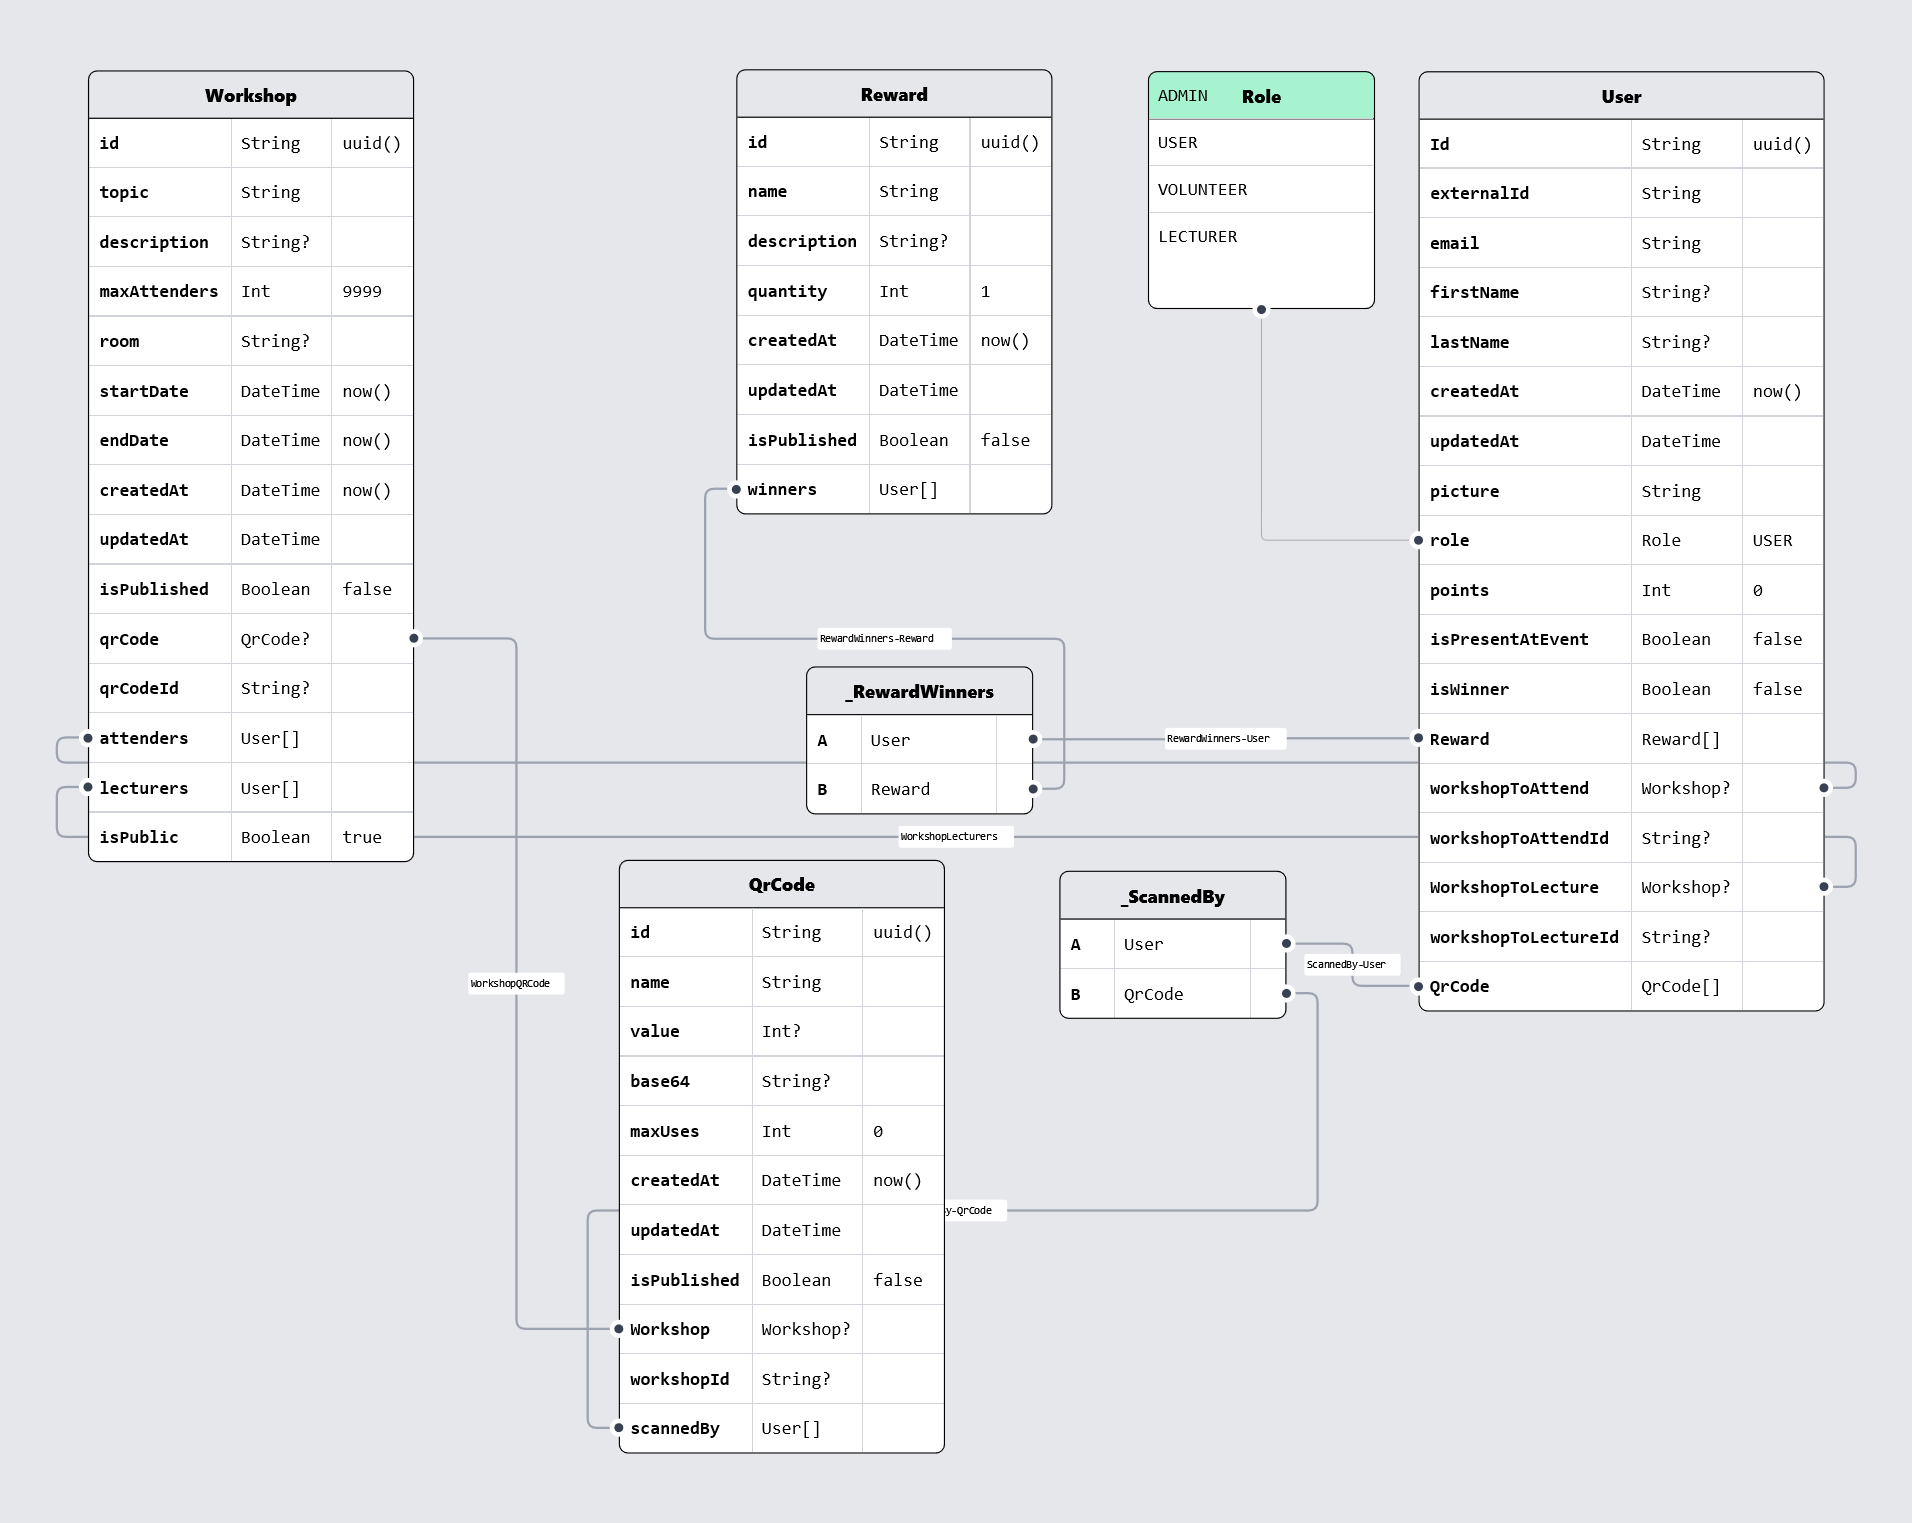
\includegraphics[scale=0.23]{imgs/database.png}
    \end{center}
    \caption{Diagram związków encji bazy danych}
    \label{db}
    \end{figure}
\noindent W bazie danych znajdują się cztery główne tabele:
\begin{itemize}
    \item \textbf{Użytkownicy} - przechowuje dane o użytkownikach aplikacji
    \item \textbf{Warsztaty} - przechowuje dane o  odbywających się warsztatach
    \item \textbf{Nagrody} - przechowuje dane o nagrodach możliwych do wygrania podczas warsztatów
    \item \textbf{Kody QR} - przechowuje dane o kodach QR mających wartość punktową
\end{itemize}

\subsubsection{Użytkownicy}
\noindent Użytkownicy to główna encja bazy danych.
\begin{itemize}
    \item \textbf{Id} - Główny klucz identyfikujący użytkownika
    \item \textbf{externalId} - Identyfikator użytkownika w systemie autoryzacji Clerk
    \item \textbf{email} - Adres email użytkownika
    \item \textbf{firstName} - Imię użytkownika
    \item \textbf{lastName} - Nazwisko użytkownika
    \item \textbf{createdAt} - Data utworzenia użytkownika
    \item \textbf{updatedAt} - Data ostatniej aktualizacji użytkownika
    \item \textbf{picture} - Adres URL do zdjęcia użytkownika
    \item \textbf{role} - Rola użytkownika w systemie (administrator, uczestnik, wolontariusz i prowadzący)
    \item \textbf{points} - Liczba zdobytych punktów przez użytkownika
    \item \textbf{isPresentAtEvent} - Zmienna logiczna określająca czy użytkownik jest obecny na wydarzeniu
    \item \textbf{isWinner} - Zmienna logiczna określająca czy użytkownik jest zwycięzcą jakiejkolwiek nagrody
    \item  \textbf{Reward} - Relacja wiele-do wielu z tabelą Nagrody. Przechowuje nagrody które użytkownik wygrał
    \item  \textbf{WorkshopToAttend} - Opcjonalna relacja z Warsztatem. Dla użytkownika który zapisał się na limitowany warsztat
    \item  \textbf{WorkshopToLecture} - Opcjonalna relacja z Warsztatem. Dla użytkownika któremu przypisano prowadzenie warsztatu
    \item  \textbf{QRCode} - Relacja wiele-do-wielu z tabelą Kody QR. Przechowuje zeskanowane kody QR przez użytkownika
\end{itemize}
\subsubsection{Warsztaty}
\noindent W tej encji przechowywane są dane o warsztatach odbywających się podczas wydarzenia.
\begin{itemize}
    \item \textbf{Id} - Główny klucz identyfikujący warsztat
    \item \textbf{topic} - Temat warsztatu
    \item \textbf{description} - Opcjonalny opis tego, co będzie się działo podczas warsztatu
    \item \textbf{MaxAttenders} - Maksymalna liczba uczestników warsztatu
    \item \textbf{room} - Sala w której odbywa się warsztat
    \item \textbf{startDate} - Data i godzina rozpoczęcia warsztatu
    \item  \textbf{endDate} - Data i godzina zakończenia warsztatu
    \item  \textbf{createdAt} - Data utworzenia warsztatu
    \item  \textbf{updatedAt} - Data ostatniej aktualizacji warsztatu
    \item  \textbf{isPublished} - Zmienna logiczna określająca czy warsztat jest upubliczniony
    \item   \textbf{QRCode} - Opcjonalna relacja jeden-do-jednego z tabelą Kody QR. Przechowuje kod QR dla warsztatu
    \item  \textbf{Lecturers} - Relacja jeden-do-wielu z tabelą Użytkownicy. Przechowuje prowadzących warsztat
    \item \textbf{Attenders} - Relacja jeden-do-wielu z tabelą Użytkownicy. Przechowuje uczestników
\end{itemize}
\subsubsection{Nagrody}
\noindent W tej encji przechowywane są dane o nagrodach możliwych do wygrani podczas wydarzenia. Losowane na podstawie punktów zebranych przez użytkowników.
\begin{itemize}
    \item \textbf{Id} - Główny klucz identyfikujący nagrodę
    \item \textbf{name} - Nazwa nagrody
    \item \textbf{description} - Opcjonalny opis nagrody
    \item \textbf{quantity} - Liczba sztuk poszczególnej nagrody
    \item \textbf{createdAt} - Data utworzenia nagrody
    \item \textbf{updatedAt} - Data ostatniej aktualizacji nagrody
    \item \textbf{isPublished} - Zmienna logiczna określająca czy nagroda jest upubliczniona
    \item \textbf{Winners} - Relacja wiele-do-wielu z tabelą Użytkownicy. Przechowuje użytkowników którzy wygrali nagrodę
    \end{itemize}
\subsubsection{Kody QR}
\noindent W tej encji przechowywane są dane o kodach QR mających wartość punktową.
\begin{itemize}
    \item \textbf{Id} - Główny klucz identyfikujący kod QR
    \item \textbf{name} - nazwa kodu QR
    \item  \textbf{value} - wartość punktowa kodu QR
    \item  \textbf{base64} - kod QR w formacie base64
    \item \textbf{createdAt} - Data utworzenia kodu QR
    \item \textbf{updatedAt} - Data ostatniej aktualizacji kodu QR
    \item \textbf{isPublished} - Zmienna logiczna określająca czy kod QR jest upubliczniony
    \item \textbf{Workshop} - Opcjonalna relacja jeden-do-jednego z tabelą Warsztaty. Przechowuje warsztat dla którego kod QR jest przeznaczony
    \item \textbf{scannedBy} - Relacja wiele-do-wielu z tabelą Użytkownicy. Przechowuje użytkowników którzy zeskanowali kod QR
    \end{itemize}
\subsection{Diagram przypadków użycia}
\input{sections/chapters/realization/przypadki.tex}
\subsection{Scenariusze przypadków użycia}
\subsection{Architektura aplikacji}

\newpage

\section{Interfejsy użytkownika}
\subsection{Strona internetowa}
\subsection{Strona główna}
\subsection{Panel administracyjny - warsztaty}
\subsection{Panel administracyjny - warsztaty}
\subsection{Aplikacja mobilna}
\newpage

\section{Podsumowanie}
Celem pracy inżynierskiej zaprojektowanie i zaimplementowanie aplikacji do zarządzania i obsługi wydarzeń uczelnianych. Cel ten został w pełni spełniony, uwzględniając wszystkie wymagania funkcjonalne i niefunkcjonalne, które zostały postawione przed systemem.

Motywacją do jej stworzenia był fakt istnienia podobnych rozwiązań, które były płatne, bądź przystosowane do dużych wydarzeń cyklicznych jak np. koncerty czy sztuki teatralne. W przypadku wydarzeń uczelnianych, które są organizowane przez koła naukowe czy studentów często nie ma możliwości na wykupienie takich rozwiązań. Dlatego też powstała aplikacja, która jest darmowa i dostępna dla każdego, kto chciałby z niej skorzystać.
\subsection {Efekt końcowy pracy}
Rezultatem wielomiesięcznej pracy jest wytworzona aplikacja. Pozwala ona na administrację wydarzeniem, zarządzanie uczestnikami, a także generowanie kodów QR. Użytkownicy mogą przeglądać nagrody, wydarzenia i się na nie zapisywać. Dodatkowo mogą skanować kody QR, które wynagradzają ich punktami. Punkty następnie  są traktowane jako losy w module losowania nagród.

Implementacja systemu pozwoliła autorowi pracy na zdobycie nowych umiejętności związanych z wytwarzaniem oprogramowania oraz poznanie nowych technologii. Pozwoliło to na rozwój umiejętności programistycznych, które będą przydatne w karierze zawodowej.

Autor pracy napotkał na kilka problemów podczas wytwarzania aplikacji. Największym z nich była współpraca z aparatem w ramach aplikacji mobilnej, w celu skanowania kodów QR. Wymagało to wielu prób i błędów, aby znaleźć rozwiązanie, które działało poprawnie. Autor nie posiadał wiedzy na temat tworzenia aplikacji mobilnej, więc wymagało to wielu godzin czytania dokumentacji.
\subsection {Możliwe kierunki rozwoju}
Projekt aplikacji posiada wiele możliwości rozwoju o funkcjonalności, które znacznie wykraczały poza zakres czasowy przeznaczony na pracę inżynierską. Większość z nich zostanie zaimplementowana przez autora pracy w ramach własnego rozwoju systemu.

Pierwszą z nich jest implementacja roli "Prowadzącego". Zapewnienie mu możliwości kontaktu z uczestnikami jego warsztatów w celu przesłania materiałów, które zostały wykorzystane podczas zajęć. Dodatkowo możliwość integracji interaktywnych quizów, które mogłyby być rozwiązane przez uczestników w czasie trwania wydarzenia, co premiowałoby dodatkowymi punktami, bądź osobnymi nagrodami - losowanymi przez prowadzącego.

Kolejną funkcjonalnością, która mogłaby zostać zaimplementowana jest interaktywna mapa. Z wykorzystaniem modułu GPS, użytkownik mógłby zobaczyć, gdzie znajduje się w stosunku do miejsca warsztatów, na które się zapisał. Następnie dotrzeć do celu, korzystając z instrukcji wyświetlanych na ekranie telefonu.

Przydatnym modułem dla systemu byłby system statystyk. Umożliwiłby on zbieranie danych i ich analizę. Dzięki temu organizatorzy mogliby sprawdzić, które wydarzenia cieszyły się największą popularnością, a które nie. Dodatkowo mogliby sprawdzić, które z nich były najczęściej odwiedzane przez użytkowników, a które nie. Dzięki temu mogliby w przyszłości lepiej planować wydarzenia, które organizują a co za tym idzie zwiększyć ilość uczestników.

Dużym potencjałem rozwoju jest również wykorzystanie kodów QR i ich skanowania w większym zakresie. Możliwe byłoby użycie ich do interakcji ze stoiskami partnerskimi i ich promocją. Rozbudowa systemu generowania kodu QR o np. umieszczanie loga partnerów w kodzie QR mogłaby przyczynić się do zwiększenia zainteresowania danym stoiskiem.

Czasem zdarza się, że wydarzenie jest odwoływane, przeniesione bądź zmodyfikowane z przyczyn niezależnych od organizatorów. W takim przypadku przydatnym modułem byłby system powiadomień. Użytkownicy, którzy zapisali się na dane wydarzenie otrzymaliby powiadomienie na swoim telefonie o zmianach, które zostały wprowadzone. Dodatkowo mogliby także otrzymywać różne informacje, które byłyby wysyłane przez organizatorów, czy przypomnienia o zbliżającym się wydarzeniu.
\newpage
\newpage

\addcontentsline{toc}{section}{Bibliografia}
\printbibliography % https://www.overleaf.com/learn/latex/Bibliography_management_in_LaTeX#Reference_guide
\newpage

\addcontentsline{toc}{section}{Spis rysunków}
\listoffigures
\newpage

\addcontentsline{toc}{section}{Spis tabel}
\listoftables
\newpage

\addcontentsline{toc}{section}{A. Załączniki}
\section*{A. Załączniki}
\input{sections/attachments}
\end{document}